\chapter{Introduction} \label{chap:introduction}

Medical diagnosis and specifically computer-aided diagnosis (CAD) is a hot topic in the field of technology. One of the main reasons for becoming a hot topic is the recent innovation and breakthroughs achieved by computer vision research. Combined with poor healthcare coverage around the globe, CAD systems offer a promising solution to mitigate the devastating impact of fatal diseases such as pneumonia. Achieving human-level accuracy in computer vision task in a wide array of classification task such as ImageNet large scale visual recognition challenge (ILSVRC)~\cite{imagenet} sparked the debates about whether these CAD systems can reduce or altogether replace the jobs such as radiologist in the future.
Controversial topics such as whether or not artificial intelligence will replace the radiologist in the future aside, these automated systems can offer answers for patient's questions in absence of medical help or to very least offer much needed second opinion in the face of unsatisfied diagnoses. Given all the mentioned possible benefits of the CAD systems, this project is focused on building classification CAD systems for diagnosing pneumonia from the chest X-ray images.

\section{Aims and Objectives} \label{sec:aimsandobj}
The aim of this project is to build a fully functional chest X-ray image classification pipeline that implements CI/CD principals to experimentation and deployment.
These pipelines also referred as MLOps where the part of the machine learning workflow is automated.

\subsection{Objectives}
Project will be implemented with execution of fallowing objectives:
\begin{enumerate}
    \item \textbf{Data pre-processing and data exploration: }Preparing the data for model ready state and general data exploration.
    \item \textbf{Building baseline model with well known neural network architectures: }This step involves setting additional benchmarks with out of the box models from section 4.
    % \item \textbf{Using pre-trained network to increase model performance: }Using pre-trained networks to help training and accuracy of the model.
    %\item Model improvement and hyper parameter tuning
    \item \textbf{Increasing model performance: }Using ensemble method and techniques such as transfer learning to increase model performance.
    %\item \textbf{Model refinement: } Prototyping for improved model thorough hyper-parameter tuning.
    %\item Saving trained model for deployment
    \item \textbf{Ensuring model interpretability with visualization: } For making sure model learning as intended and focusing on correct parts of the image.
    \item \textbf{Applying different deployment options: } Implementation of model development. Based on best choice for project specification.
\end{enumerate}
It's worth emphasizing that the objective of this project is not to achieve the state of the art result in pneumonia detection but to offers a preferred method for improving and enhancing the existing models.
The intuition behind choosing the above objectives instead of attempting to build novel architecture from scratch is the process of choosing a novel architecture has a very large search space and requires a lot of iteration and experimentation. Due to the limited time frame of this project attempting to find new architecture would not be feasible. Additionally, objectives designed to serve the project goal with consistent aims. For example, item 1 and 2 will focus on reducing the model over-fitting while item 5 would serve as a tool to detect over-fitting. Objective 2 serves as a selection for a suitable model and setting benchmark while 6 is aimed at improving the model.

\section{CI/CD Pipeline} \label{sec:cicd}
In this section, I will give a brief introduction to the CI/CD pipeline to explain what CI/CD is and why it is chosen as a preferred way to build this project.

Continuous integration (CI) is a workflow strategy that helps ensure everyone's changes will integrate with the current version of the project in the typical software engineering team. This lets members of the team catch bugs, reduce merge conflicts, and increase overall confidence that your software is working. While the details may vary depending on the development environment, most CI systems feature the same basic tools and processes. In most scenarios, a team will practice CI in conjunction with automated testing using a dedicated server or CI service. Whenever a developer adds new work to a branch, the server will automatically build and test the code to determine whether it works and can be integrated with the code on the main development branch. The CI server will produce output containing the results of the build and an indication of whether or not the branch passes all the requirements for integration into the main development branch. By exposing build and test information for every commit on every branch, CI paves the way for what's known as continuous delivery, or CD, as well as a related process, called continuous deployment. The difference between continuous delivery and continuous deployment is that CD is the practice of developing software in such a way that you could release it at any time. When coupled with CI, continuous delivery lets you develop features with modular code in more manageable increments. Continuous development is an extension of continuous delivery. It's a process that allows you to actually deploy newly developed features into production with confidence, and experience little if any, downtime. Even though the benefits of using CI/CD pipelines are more prominent in the software teams, integration automated testing will help even individual projects such as this by reducing time for debugging.

In more granular detail, this system works with central version control services and in this project central version control service used is Github. GitHub uses a communication tool called \emph{webhooks} to send messages to external systems about activities and events that occurred in the project. For each event type, subscribers will receive messages related to the event. Generally, events refer to action involving the software such as new commit push, pull (merge) request, or other software related action. In this case, whenever a new commit is pushed to any branch of the project, a message from Github will be sent out to a third party system called \emph{travis.}~\footnote{https://travis-ci.org/} Travis is a hosted CI service that allows build and test software hosted in version control services. When travis receives the webhook call it will fetch the most recent version of the project and run the tests associated with it. When the test runs completed with the latest version of the software, test results will be sent back to relevant commits as status information using GitHub API. This information can either be used by developers for making decisions such as whether to accept the pull request versus reject it or if applicable can be used by service to initiate the deployment process for the software. In all cases, CI/CD will work as automation for software quality assurance process to speed up the development and improve the overall reliability of the software.

\begin{figure}[H]
    \centering
    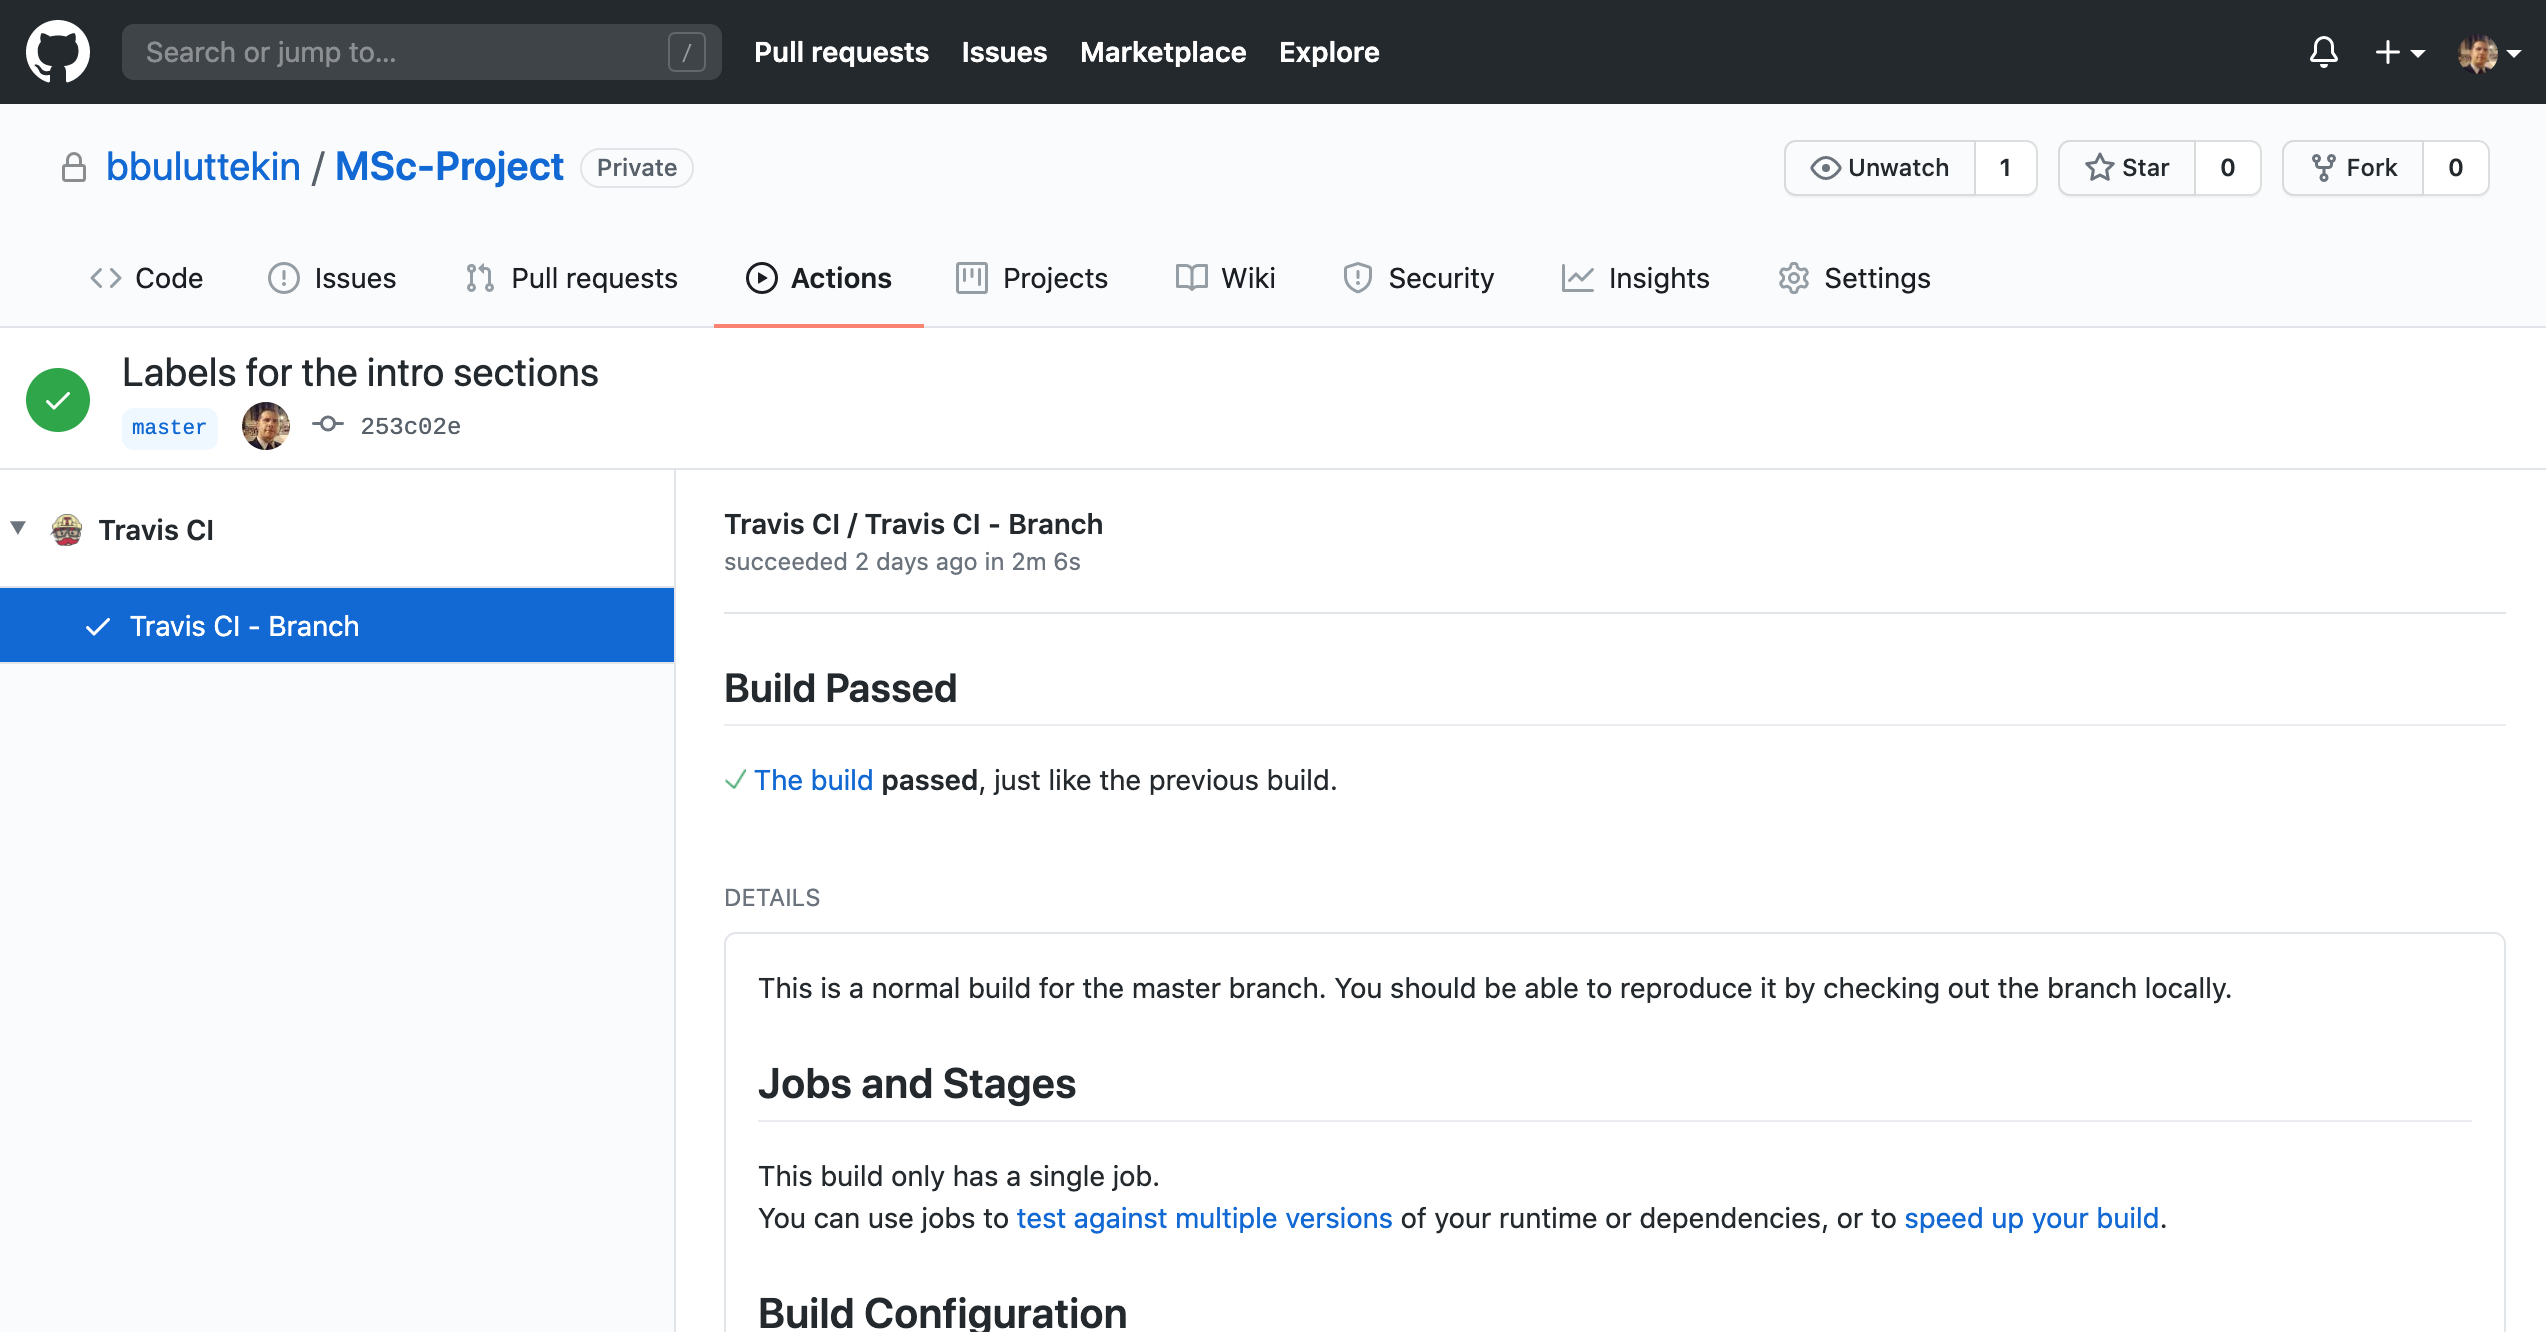
\includegraphics[width=\textwidth]{img/cigithub.png}
    \caption{CI feedback received from Travis.}
    \label{fig:cigithub}
\end{figure}
 


\section{Project specification and design} \label{sec:projectlayout}
This project I aimed to keep code and reporting together to provide easy reproduction. Codebase design to be extendable and modular. Therefore, I assign a sub-folder for all the project-specific code under the name \emph{src}. Having a module in the same directory level with the other components allows the ability to use the code in notebook experiment as well as with the tests in the CI integration.
Both project proposal and report developed using the LaTeX typesetting system and documents kept in the version controlling to allow easy changes and rolling back to the desired version. Finally, root-level files such as \emph{.travis.yml} and \emph{requirements.txt} is instrumental in defining which steps to take in CI runs and constructing a near-identical environment for software dependencies.
Below, I added a directory tree to serve as a guide for navigating and finding project files.

\dirtree{%
.1 .
.2 Proposal.
.3 Proposal files.
.2 Report.
.3 chapters.
.4 Chapter files.
.3 img.
.4 Images.
.3 Main project latex files.
.2 scripts.
.3 Utility scripts.
.2 notebooks.
.3 Experiment notebooks.
.2 src.
.3 Python library files.
.2 tests.
.3 Test files.
.2 .gitignore.
.2 .travis.yml.
.2 README.md.
.2 requirements.txt.
}

\section{Reproducibility Guidance} \label{sec:reproducibility}
As a scientific project, it is very important that anyone can reproduce the experiments and findings in this project to verify the conclusions reached are accurate. Main components of reproducible research are open code, open data and repeatable software runtime specification. Open code component is the most straightforward among the other components as the source-code produced part of this project will be shared with the project reviewers and will be made public in GitHub~\footnote{https://github.com/bbuluttekin/MSc-Project} once the assessment of the project is completed. Dataset~\cite{dataset} used in this project is also available through the website URL cited and hosted in online data science community called Kaggle~\footnote{https://www.kaggle.com/paultimothymooney/chest-xray-pneumonia}. I have used Kaggle as the main source of accessing this data for two reasons, firstly for its functionality of allowing API calls to retrieve data and secondly for managing the data versioning for the user. Data versioning is an integral component of the reproduction of machine learning projects because the model produced by the training will heavily depend on the data it trained. 
The current version of the dataset as of the writing of this project is version 2. 
To enable easier runtime replication and to leverage computational power I have chosen to use an online service called Google Colaboratory.~\footnote{https://colab.research.google.com/} Colaboratory or \emph{"Colab"} for short is a free service provided by Google Research. It will allow running Python code through the browser that connected to remote compute resources. Considering that Colab is a remote compute resource, I have created starter utility scripts to automate data acquisition. These files can be found inside the \emph{scripts} folder. Please note that using these script will require obtaining API key from Kaggle platform and this API key file should be in the path specified in the scripts. However, reproducing in the Colab is optional and software dependencies required to produce local development environment is provided with the "requirements.txt" file. Lastly, custom software components for this project resides in the "src" folder and this folder must be placed in a location available to the scope of the python runtime.


\clearpage